% Autore originale: Fabio Tempera
% Licenza: MIT (vedere LICENSE nel medesimo direttorio)
%
% DOCUMENTO
%   Proposta di partecipazione alla rete TESS-4C per gruppi astrofili.
%
% COMPILAZIONE
%   pdflatex gruppi-astrofili.tex  (due passate per i riferimenti)
%   Classe report, pacchetti in packages.sty. Non usare Markdown.

\documentclass[11pt,a4paper]{report}

\usepackage{packages}

\definecolor{nightblue}{RGB}{22,38,58}
\definecolor{steel}{RGB}{80,100,120}
\definecolor{linegray}{RGB}{200,200,200}

\renewcommand{\thesection}{\arabic{section}}
\setcounter{secnumdepth}{0}

\titleformat{\section}
  {\normalfont\Large\bfseries\color{nightblue}}
  {\thesection}{0.6em}{}
\titlespacing{\section}{0pt}{1.4em}{0.6em}

\pagestyle{fancy}
\fancyhf{}
\renewcommand{\headrulewidth}{0.4pt}
\renewcommand{\headrule}{\hbox to\headwidth{\color{linegray}\leaders\hrule height \headrulewidth\hfill}}
\fancyhead[L]{\small\color{steel} CieloBuio OdV}
\fancyhead[R]{\small\color{steel} Rete TESS-4C, proposta per gruppi astrofili}
\fancyfoot[C]{\small\color{steel}\thepage}

\hypersetup{
  colorlinks=true,
  urlcolor=nightblue,
  pdftitle={Rete TESS-4C. Proposta per gruppi astrofili},
  pdfauthor={Fabio Tempera}
}

\setlist[itemize]{leftmargin=1.4em, itemsep=0.25em, topsep=0.3em}

\begin{document}

\begin{center}

{\LARGE\bfseries\color{nightblue} Una stazione per il monitoraggio del cielo notturno\par}

\vspace{0.2cm}

{\large Proposta di partecipazione per gruppi astrofili\par}

\vspace{0.1cm}

{\small CieloBuio OdV, progetto rete TESS-4C}

\end{center}

\section*{Oggetto}

Questo documento presenta una rete di stazioni per la misura della qualità del cielo notturno, in via di costituzione in Italia nell'ambito del progetto TESS-4C di CieloBuio OdV. Lo scopo è verificare il grado di interesse dei gruppi astrofili a dotarsi in autonomia di uno strumento di misura che entrerebbe a far parte della rete.

\section*{L'inquinamento luminoso}

L'inquinamento luminoso è l'alterazione della quantità e della distribuzione della luce artificiale nelle ore notturne. Il fenomeno è nato nella comunità astronomica, preoccupata che la luce artificiale rendesse sempre più difficile osservare il cielo stellato. Oggi lo stesso tema interessa l'ecologia, perché la luce notturna modifica i ritmi di vita di molte specie animali e vegetali, e interessa il risparmio energetico, perché un'illuminazione superflua o mal orientata comporta costi evitabili.

Il passaggio dalle lampade tradizionali ai LED ha reso l'illuminazione più efficiente, ma ha anche modificato la composizione spettrale della luce emessa, con una maggiore quota di blu. Un'efficienza più alta non ha ridotto automaticamente la luce complessiva: in molti casi l'illuminazione è aumentata, e i suoi effetti si estendono ben oltre la sorgente.

Si stima che circa il 99\% della popolazione di Stati Uniti ed Europa viva sotto un cielo inquinato, e che più del 33\% della popolazione mondiale non possa più osservare la Via Lattea (Falchi et al., 2016). Per valutare l'efficacia delle norme regionali sul contenimento della luce artificiale servono dati oggettivi misurati a terra, perché le stime da satellite non sono sufficientemente puntuali.

\section*{Lo strumento TESS-4C}

Il TESS-4C è un fotometro a 4 bande, sviluppato nell'ambito del progetto STARS4ALL. Misura la brillanza del cielo e trasmette i dati via WiFi. Le misure confluiscono nell'archivio aperto della rete STARS4ALL e in un cruscotto gestito da CieloBuio OdV.

\section*{Cosa cambierebbe per un gruppo astrofilo}

Per un gruppo astrofilo la stazione diventa una fonte di dati continui sulla brillanza del cielo nel proprio territorio. Le serie possono accompagnare le serate osservative, documentare nel tempo le condizioni di osservazione e sostenere l'attività di divulgazione verso il pubblico. Il gruppo resta autonomo nella scelta del punto di installazione, nel rispetto dei requisiti tecnici, e nelle iniziative che ne derivano.

\section*{Cosa offriamo}

CieloBuio OdV collega lo strumento alla rete STARS4ALL, raccoglie le misure e le rende consultabili in un cruscotto di sintesi. Offre inoltre un supporto a distanza per la configurazione. La sede, l'installazione e la connessione restano a cura del soggetto ospitante.

\section*{Il sito di installazione}

Lo strumento va installato in un punto con zenit libero e privo di luce artificiale diretta, come un lampione o un'insegna. Sono inoltre necessarie un'alimentazione a 5\,V e una copertura WiFi. La Figura~\ref{fig:installazione} confronta una geometria non idonea, con il fotometro esposto al lampione, e una geometria idonea, con il fotometro al centro del tetto e il lampione schermato dall'edificio. La verifica va fatta in situ, di notte, prima del fissaggio definitivo.

\begin{figure}[ht!]
\centering

\begin{tabular}{@{}cc@{}}
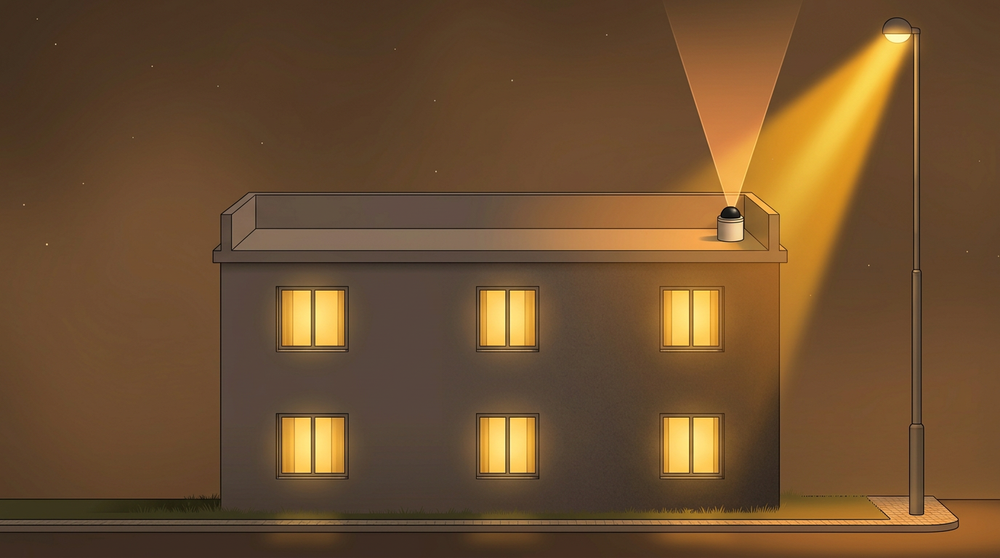
\includegraphics[width=0.48\textwidth]{figures/installazione_non_idonea.png} &
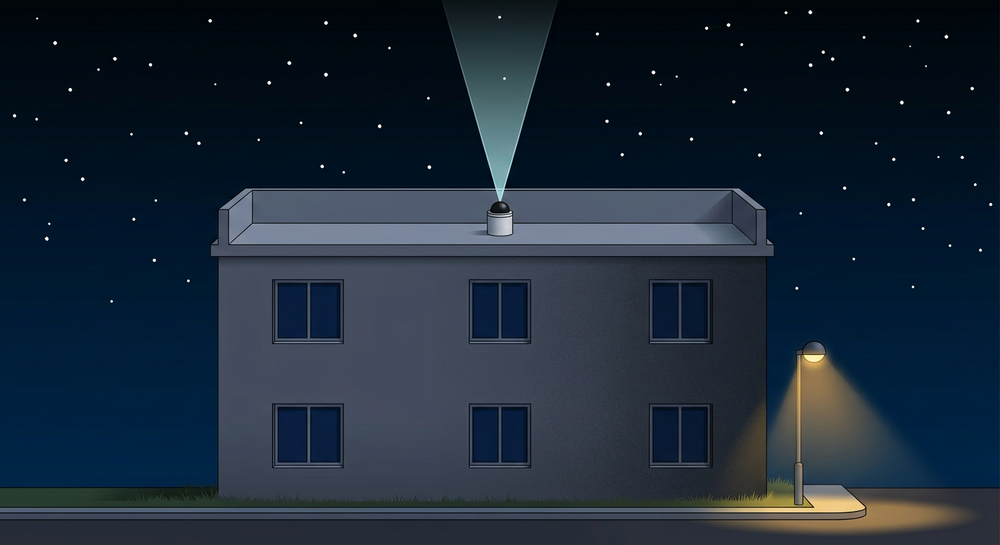
\includegraphics[width=0.48\textwidth]{figures/installazione_idonea.png}
\end{tabular}

\caption{Installazione del fotometro: geometria non idonea (sinistra) e geometria idonea (destra).}
\label{fig:installazione}
\end{figure}

\section*{La proposta}

Vi interesserebbe far parte di questa rete? Il gruppo acquisterebbe in autonomia uno strumento, al costo indicativo di 550-650 EUR con IVA e spedizione comprese, lo installerebbe in un punto con cielo libero dallo zenit e privo di luce artificiale diretta, e lo manterrebbe nel tempo. Lo strumento resterebbe nella disponibilità del gruppo.

Una risposta di interesse non comporta alcun impegno di acquisto. Dopo le prime risposte è prevista una riunione online di circa 30 minuti, dedicata a illustrare il progetto nel dettaglio e a definire i passaggi successivi.

\section*{Per informazioni}

Per rispondere o chiedere chiarimenti è possibile scrivere a \url{fabiot2801@gmail.com} oppure inviare un messaggio WhatsApp al numero 329 883 5142, indicando il nome del soggetto interessato e un referente.

\vspace{0.6cm}

\noindent Fabio Tempera, CieloBuio OdV

\end{document}
